\section{Влияние порядка обхода на скорость сходимости} \label{ch3:order}
	Как было сказано в главе \ref{ch2:xpbd}, одним из недостатков алгоритма PBD является его зависимость от порядка обхода ограничений. При этом, алгоритм XPBD не решает этой проблемы. Авторами статьи \cite{muller2020detailed} предлагается использовать алгоритм основанный на методе Якоби (\firef{alg:projectConstraintsJacobi}), однако данный метод на практике является менее стабильным. Автором данной работы было принято решение изучить влияние порядка обхода на скорость сходимости алгоритма PBD. Стоит отметить, что данное исследование также может быть применимо на алгоритм XPBD, так как в случае бесконечной жесткости эти два алгоритма совпадают.
	
	Для начала введем понятие \say{веревки} - тривиальный случай ткани, в котором частицы связаны друг с другом ограничениями типа \say{пружина} последовательно, как представленно на \firef{fig:rope}.
	
	\begin{figure}[ht!] 
		\center
		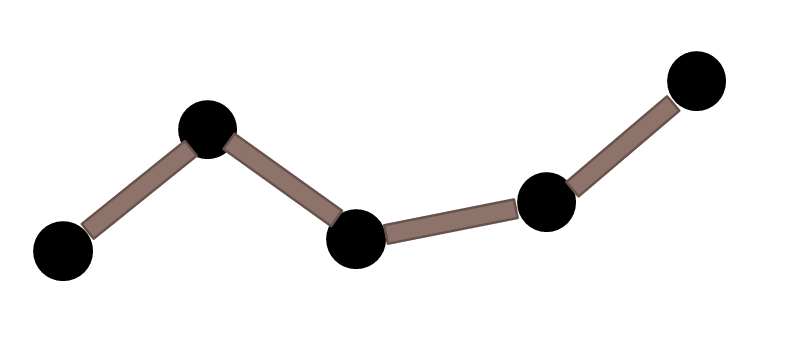
\includegraphics [scale=0.3] {my_folder/images//rope}
		\caption{Пример веревки. Черным обозначены частицы, коричневым обозначены ограничения}
		\label{fig:rope}  
	\end{figure}
	
	Проверим экспериментальным образом, имеется ли влияние порядка обхода на сходимость. Для этого поставим следующий эксперимент:
	\begin{itemize}
		\item Рассматривается одномерное пространство
		\item В данном пространстве помещается веревка, состоящая из 4-х вершин
		\item Крайняя левая частица оттягивается от остальных частиц и закрепляется в пространстве
		\item Рассматривается работа первой итерации алгоритма PBD, с двумя разными обходами. Первый - слева-направо, второй справа-налево.
	\end{itemize}
	
	\begin{figure}[ht!] 
		\center
		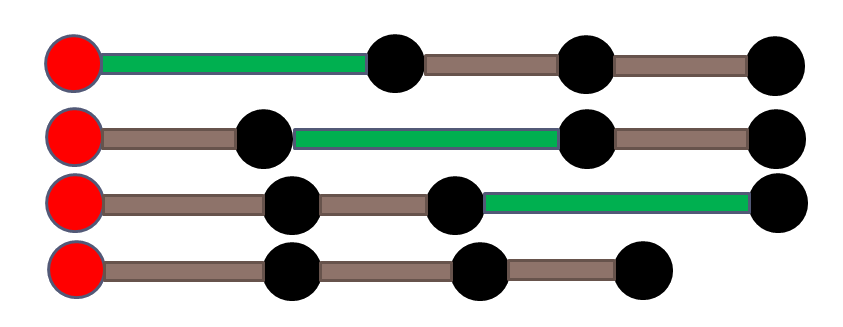
\includegraphics [scale=0.35] {my_folder/images//experiment_forward.png}
		\caption{Эксперимент с обходом слева-направо. Сверху-вниз представлены состояния веревки на каждом шаге первой итерации алгоритма PBD. Черным обозначены частицы, коричневым обозначены ограничения. Красным обозначена закрепленная частица, зеленым обозначено ограничение, которое будет обрабатываться следующим.}
		\label{fig:experiment-forward}  
	\end{figure}

	\begin{figure}[ht!] 
		\center
		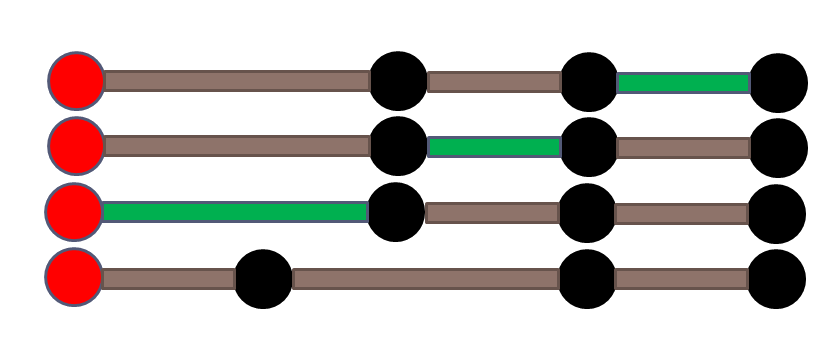
\includegraphics [scale=0.35] {my_folder/images//experiment_backward.png}
		\caption{Эксперимент с обходом справа-налево. Сверху-вниз представлены состояния веревки на каждом шаге первой итерации алгоритма PBD. Черным обозначены частицы, коричневым обозначены ограничения. Красным обозначена закрепленная частица, зеленым обозначено ограничение, которое будет обрабатываться алгоритмом.}
		\label{fig:experiment-backward}  
	\end{figure}	
	
	Из экспериментов, продемонстрированных на \firef{fig:experiment-forward} и \firef{fig:experiment-backward} можно заметить, что обход слева-направо(\firef{fig:experiment-forward}) позволяет за первую итерацию перенести растяжение с первого ограниченичения до последнего, и убрать его полностью за счет крайней правой вершины. С другой стороны, обход справа-налево(\firef{fig:experiment-backward}) за первую итерацию перенес растяжение только на второе ограничение. Стоит отметить, что данный эксперимент совпадает с результатами обнаруженными в \cite{gu2017constraint}.
	
	Однако данный эксперимент показывет только влияние двух обходов, и только на первую итерацию алгоритма. В связи с этим, поставим следующий эксперимент.
	
	\begin{itemize}
		\item Рассматривается одномерное пространство
		\item В данном пространстве помещается веревка с бесконечной жесткостью, состоящая из $N$ частиц
		\item Каждая частицы находится на расстоянии $1$ относительно других вершин.
		\item Для каждого ограничения расстояние покоя принимается за $1$
		\item Крайняя левая вершина оттягивается от остальных вершин и закрепляется в пространстве таким образом, чтобы быть на расстоянии $2$ от второй вершины.
		\item Рассматриваются следующие обходы
			\begin{enumerate}[1.]
				\item $forward$ - обход слева-направо
				\item $backward$ - обход справа-налево
				\item $shuffle$ - каждая четная итерация запускается по обходу $forward$, каждая нечетная итерация запускается по обходу $backward$
				\item $random$ - на каждой итерации список ограничений перемешивается и проходится в случайном порядке
				\item $coloring$ - сначала обходятся ограничения с четными номерами, затем ограничения с нечетными номерами
			\end{enumerate}
		\item Запускается алгоритм PBD с разными наборами параметров, и считается сколько итераций необходимо, для того чтобы веревка была обсчитана
		\item Веревка считается обсчитанной, если сумма модулей значений функций ограничений стала меньше, чем $10^{-5}$
	\end{itemize}
	
	Данный эксперимент был поставлен с использованием языка программирования Python. Результаты данного эксперимента указаны в \taref{tab:order-experiment}
	
	\noindent % for correct centering
	\begin{minipage}{\textwidth}
		\vspace{\mfloatsep} % интервал 
		\centering\small
		\captionof{table}{Результаты эксперимента применения различных обходов для различных веревок в одномерном пространстве)}%
		\label{tab:order-experiment}
		\begin{tabular}{|l|l|c|}
			\hline
			\textbf{N} & \textbf{Порядок обхода} & \textbf{Количество итераций} \\
			\hline
			$4$ & $forward$ & $41$  \\ \hline
			$4$ & $backward$ & $43$ \\ \hline
			$4$ & $shuffle$ & $63$  \\ \hline
			$4$ & $random$ & $51$   \\ \hline
			$4$ & $coloring$ & $42$ \\ \hline
			$8$ & $forward$ & $229$  \\ \hline
			$8$ & $backward$ & $235$ \\ \hline
			$8$ & $shuffle$ & $278$  \\ \hline
			$8$ & $random$ & $293$   \\ \hline
			$8$ & $coloring$ & $232$ \\ \hline
			$16$ & $forward$ & $1064$  \\ \hline
			$16$ & $backward$ & $1078$ \\ \hline
			$16$ & $shuffle$ & $1156$  \\ \hline
			$16$ & $random$ & $1353$   \\ \hline
			$16$ & $coloring$ & $1071$ \\ \hline
			$32$ & $forward$ & $4562$  \\ \hline
			$32$ & $backward$ & $4592$ \\ \hline
			$32$ & $shuffle$ & $4738$  \\ \hline
			$32$ & $random$ & $5749$   \\ \hline
			$32$ & $coloring$ & $4577$ \\ \hline
			$64$ & $forward$ & $18876$  \\ \hline
			$64$ & $backward$ & $18938$ \\ \hline
			$64$ & $shuffle$ & $19222$  \\ \hline
			$64$ & $random$ & $23746$   \\ \hline
			$64$ & $coloring$ & $18907$ \\ \hline	
		\end{tabular}
		\vspace{\mfloatsep} % интервал 
		\normalsize %восстанавливаем шрифт 	
	\end{minipage}
	
	Исходя из представленных данных, можно сделать следующие выводы
	\begin{enumerate}[1.]
		\item Порядок обхода влияет на количество итераций
		\item Размер веревки влияет на количество итераций
		\item Наблюдается квадратичная зависимость количества итераций от количества частиц
		\item Порядок обхода влияет на количество итераций много меньше, чем количество частиц
		\item Наиболее оптимальным с точки зрения количества итераций является обход $forward$ что соответствует наблюдению в работе \cite{gu2017constraint}
		\item Вторым по оптимальности является обход $coloring$
	\end{enumerate}
	
	Стоит отметить, что обход $forward$, несмотря на то что является оптимальным по количеству итераций, не может быть распараллелен.В свою очередь, обход $coloring$, основанный на принципе реберной раскраски графа, может быть распараллелен, так как в силу определения реберной раскраски, никакие два ребра одного цвета не имеют общих вершин. Это означает, что можно параллельно запустить обсчёт всех ребер одного цвета, тем самым уменьшив время работы одной итерации. 

%% Вспомогательные команды - Additional commands
%
%\newpage % принудительное начало с новой страницы, использовать только в конце раздела
%\clearpage % осуществляется пакетом <<placeins>> в пределах секций
%\newpage\leavevmode\thispagestyle{empty}\newpage % 100 % начало новой страницы